\FloatBarrier
\subsection{LS identification with white noise on output}
We modify the Simulink model and Matlab codes from the previous section to include a white noise on the output. Amplitude of the output noise is set to be $0.1$ of the actual output of the system. \autoref{code:LSIWNOOutputNoiseGeneration} is required Matlab code to generate the desired output noise.
\autoref{fig:LSIWNOSineSimulinkModel} and \autoref{fig:LSIWNONoiseSimulinkModel} are Simulink models for system with a sine input and white noise input.

\begin{figure}
	\centering
	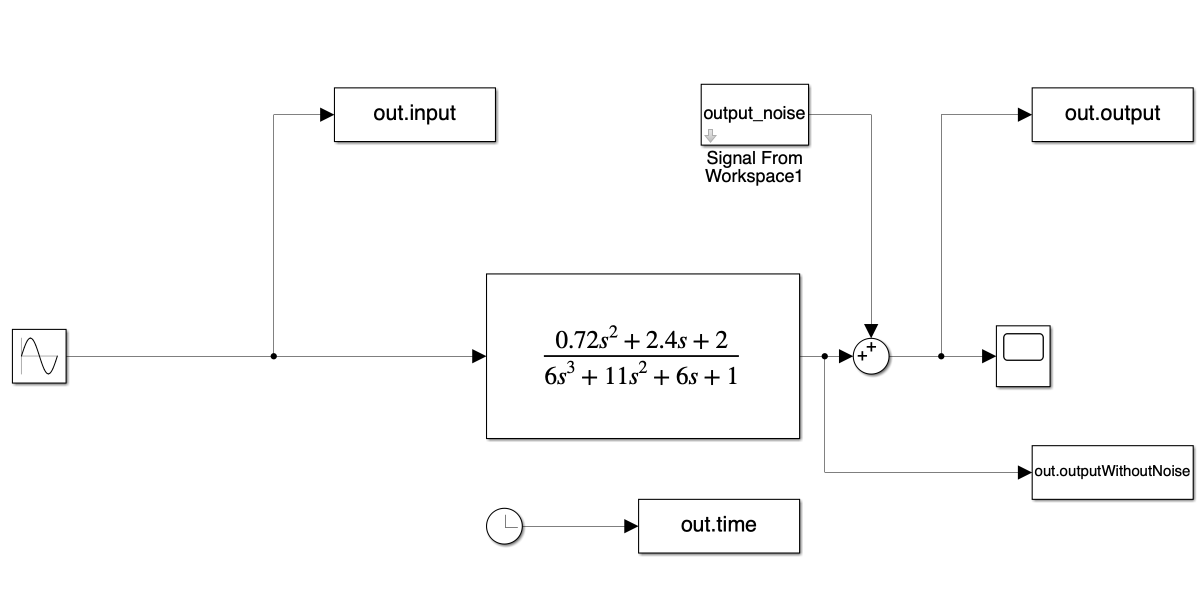
\includegraphics[totalheight=8cm]{images/LSIWNOSineSimulinkModel.png}
	\caption{Simulink model with sine input and white noise on output}
	\label{fig:LSIWNOSineSimulinkModel}
\end{figure}

\begin{figure}
	\centering
	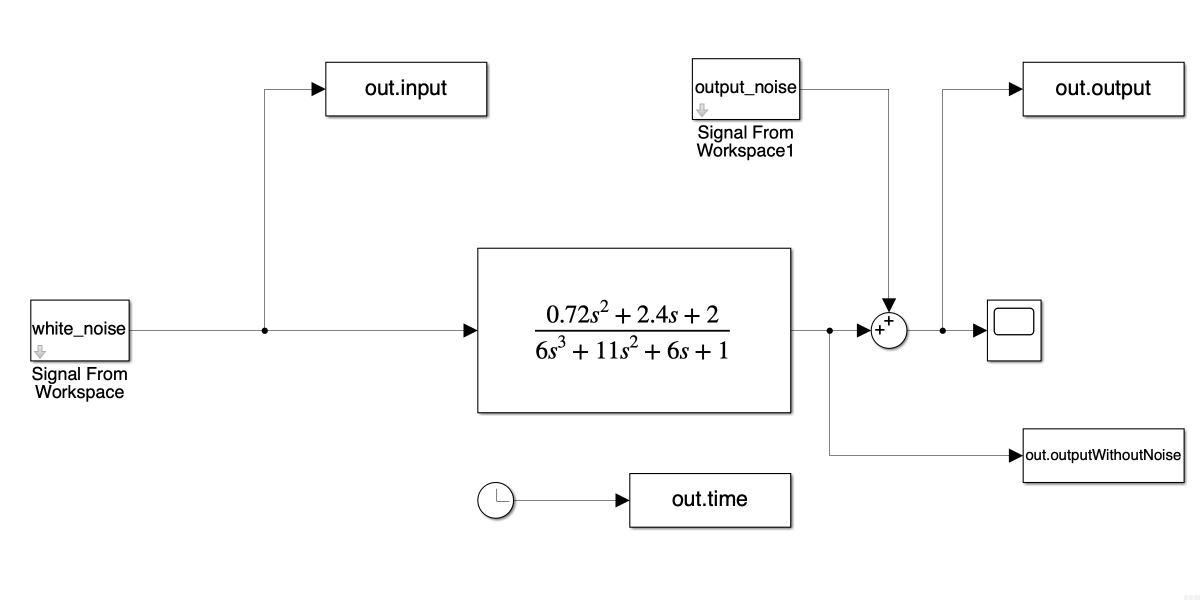
\includegraphics[totalheight=8cm]{images/LSIWNONoiseSimulinkModel.png}
	\caption{Simulink model with white noise input and white noise on output}
	\label{fig:LSIWNONoiseSimulinkModel}
\end{figure}

\begin{code}
	\begin{matlabcode}{firstnumber = 4}
%% Generate output noise 
signal_length = 3334; 
desired_output_variance = 1; 
output_noise = randn(signal_length, 1);
current_output_variance = var(output_noise);
output_scaling_factor = sqrt(desired_output_variance / current_output_variance);
output_noise = output_noise * output_scaling_factor;
output_noise = normalize(output_noise, 'range', [-0.375 0.375]);
actual_output_variance = var(output_noise);
	\end{matlabcode}
	\captionof{listing}{Output white noise generation in Matlab}
	\label{code:LSIWNOOutputNoiseGeneration}
\end{code}

We compare the identified system's output with the actual output (without noise) of the system. \autoref{fig:LSIWNOSineOutputVSSimulated} shows the output of the simulated system model versus the actual system output when a sine wave is use as input. \autoref{fig:LSIWNONoiseOutputVSSimulated} shows the output of the simulated system model versus the actual system output when a white noise is used as input.

\begin{figure}
	\centering
	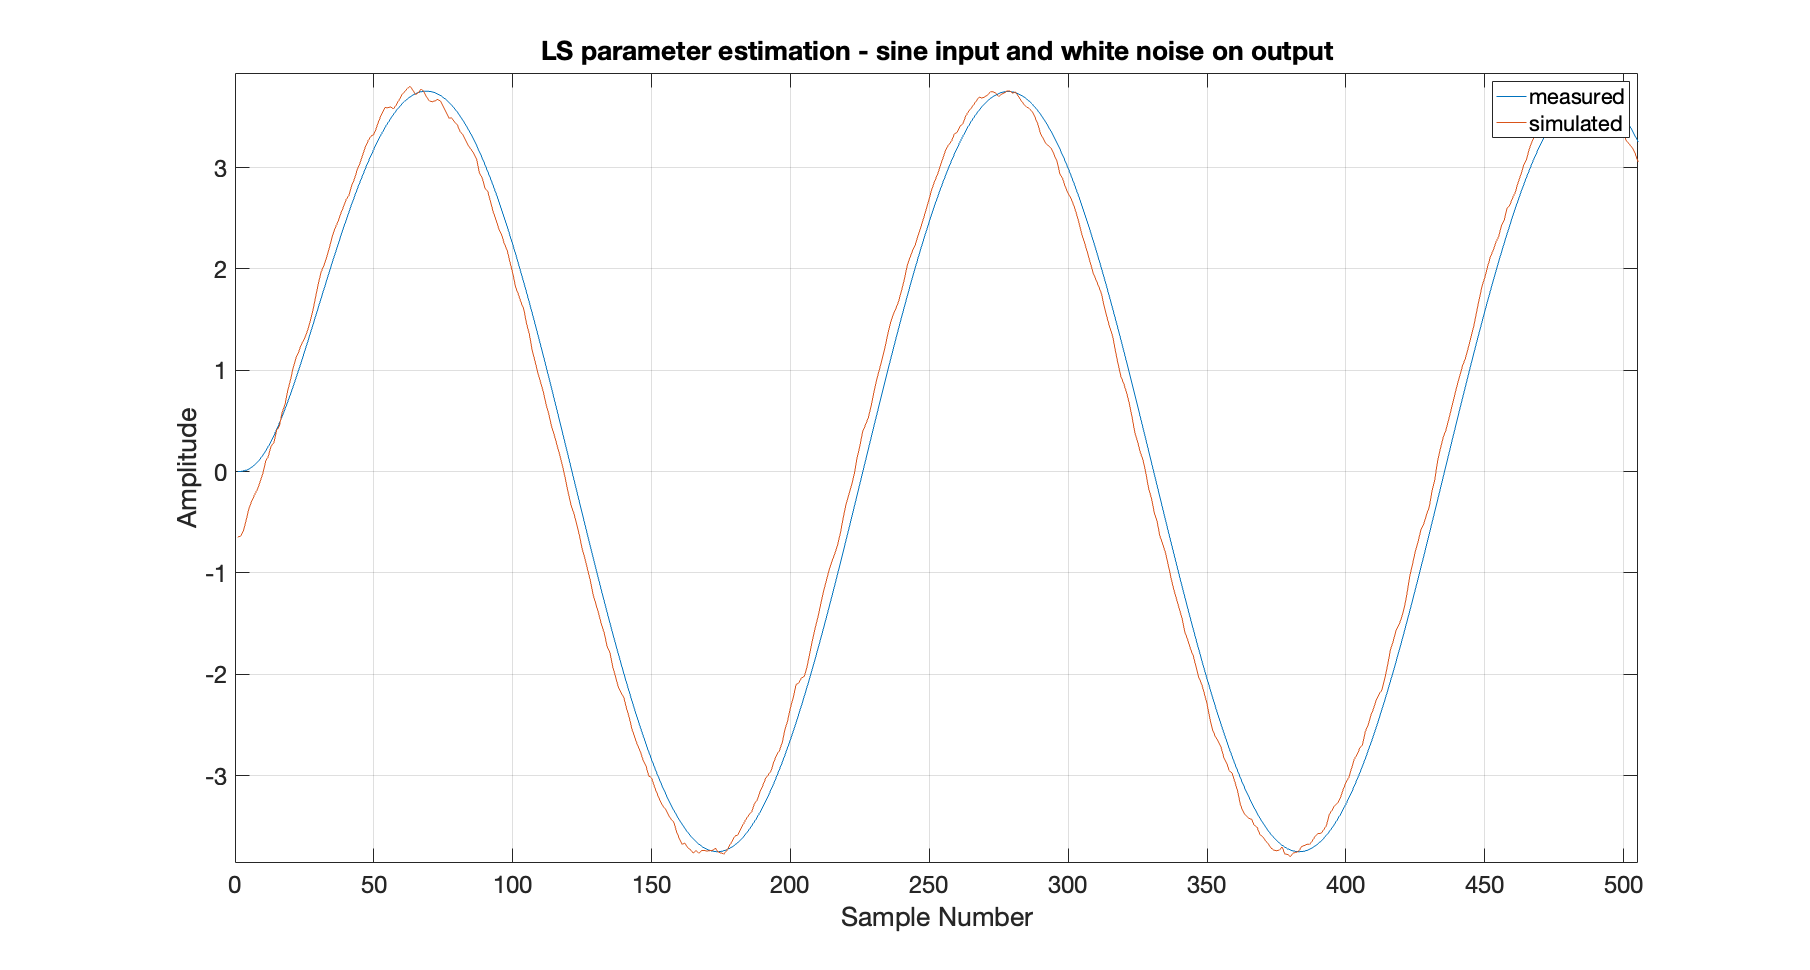
\includegraphics[totalheight=8cm]{images/LSIWNOSineOutputVSSimulated.png}
	\caption{LS system output comparison for sine input \& white noise on output}
	\label{fig:LSIWNOSineOutputVSSimulated}
\end{figure}
\begin{figure}
	\centering
	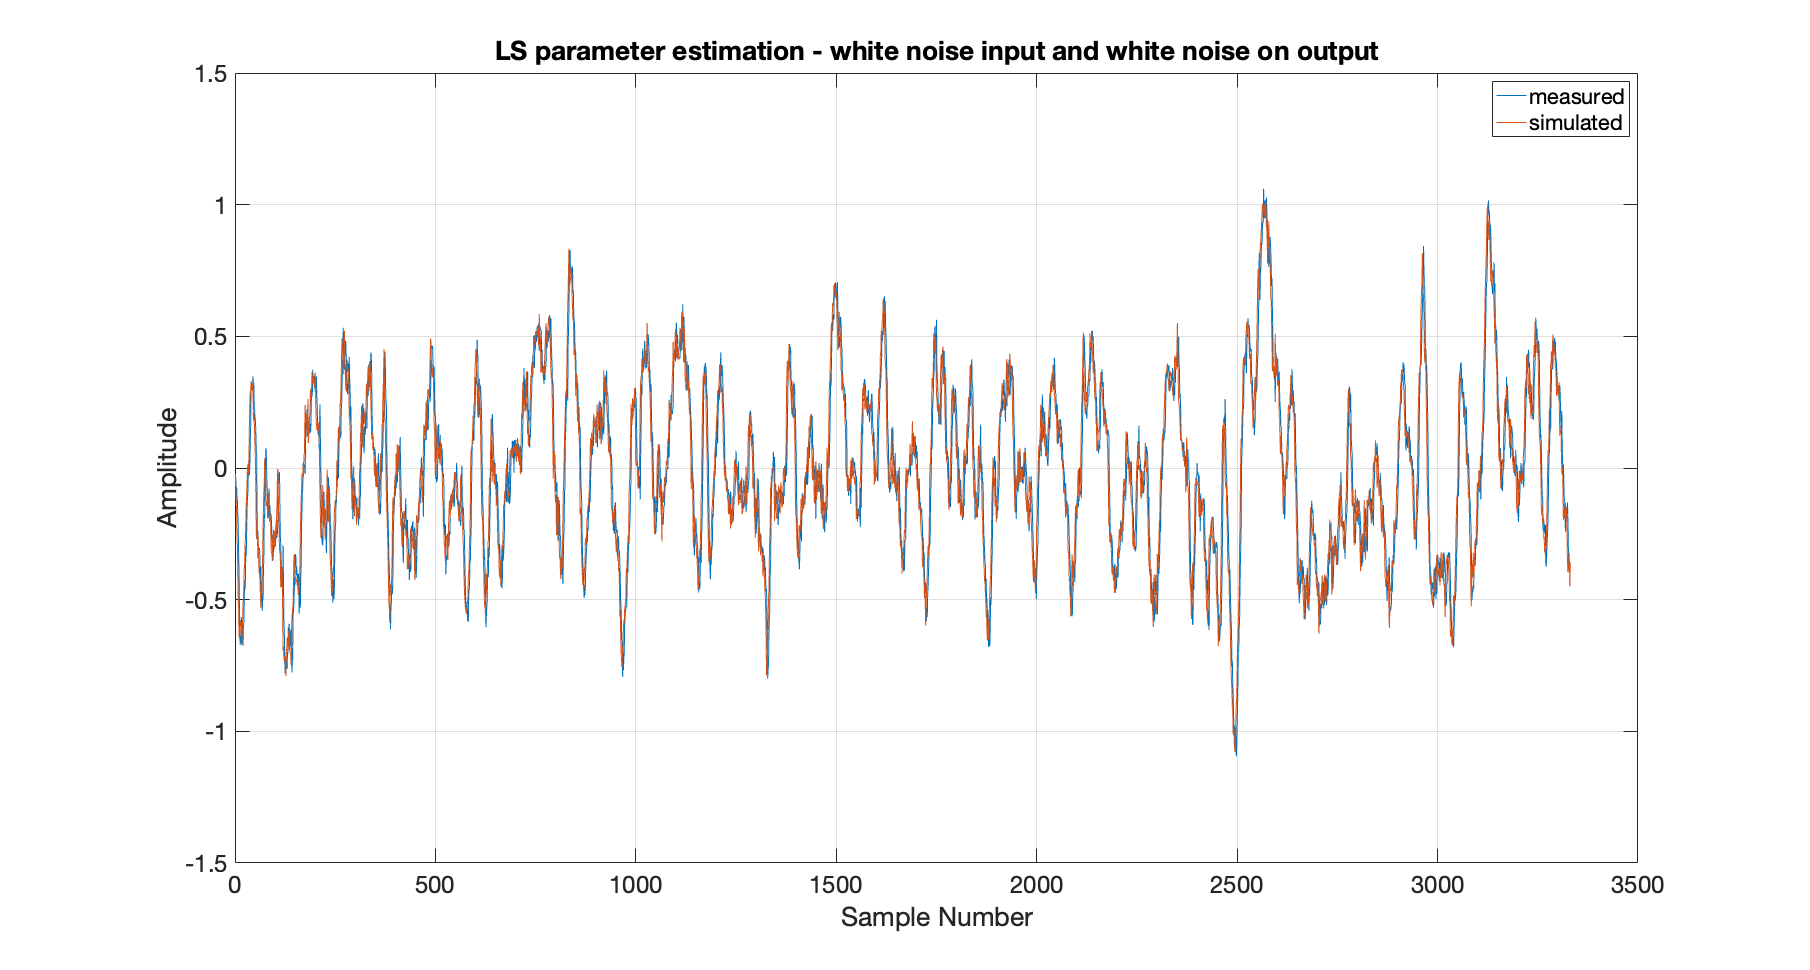
\includegraphics[totalheight=8cm]{images/LSIWNONoiseOutputVSSimulated.png}
	\caption{LS system output comparison for white noise input \& white noise on output}
	\label{fig:LSIWNONoiseOutputVSSimulated}
\end{figure}

Because of the noise on the output of the system, The MSE is much higher and has a magnitude of $10^{-3}$ (example: 0.0014). \autoref{eq:LSIWNOSineInput} shows the identified system transfer function for sine inputed system and \autoref{eq:LSIWNONoiseInput} demonstrates the transfer function of the identified system with white noise input.


\begin{equation}
	G(z) =	\frac{-4.686 z^2 + 0.2784 z + 5.242}{z^3 - 0.1968 z^2 - 0.1637 z - 0.1684}
	\label{eq:LSIWNOSineInput}
\end{equation}

\begin{equation}
	G(z) =	\frac{0.04364 z^2 + 0.0236 z + 0.008192}{z^3 - 0.7608 z^2 - 0.3535 z + 0.1425}
	\label{eq:LSIWNONoiseInput}
\end{equation}

The Simulink model and Matlab code for the sine input system are located at  \hspace{-1ex}\lstinline| assignment1/part1/1_2/LS1_2_sine.m| and  \hspace{-1ex}\lstinline| assignment1/part1/1_2/LS1_2_SN.slx|.The white noise input system model and code are located at  \hspace{-1ex}\lstinline| assignment1/part1/1_2/LS1_2_noise.m| and  \hspace{-1ex}\lstinline| assignment1/part1/1_2/LS1_2_NS.slx|.
